\documentclass[a4paper]{article}

\usepackage[T1]{fontenc}
\usepackage[utf8]{inputenc}
\usepackage{mlmodern}

%\usepackage{ngerman}	% Sprachanpassung Deutsch

\usepackage{graphicx}
\usepackage{geometry}
\geometry{a4paper, top=15mm}

\usepackage{subcaption}
\usepackage[shortlabels]{enumitem}
\usepackage{amssymb}
\usepackage{amsthm}
\usepackage{amsmath}
\usepackage{mathtools}
\usepackage{braket}
\usepackage{bbm}
\usepackage{graphicx}
\usepackage{float}
\usepackage{yhmath}
\usepackage{tikz}
\usepackage{scratch}
\usetikzlibrary{patterns,decorations.pathmorphing,positioning}
\usetikzlibrary{calc,decorations.markings}

\usepackage[backend=biber, sorting=none]{biblatex}
\addbibresource{cite.bib}

\usepackage[framemethod=TikZ]{mdframed}

\tikzstyle{titlered} =
    [draw=black, thick, fill=white,%
        text=black, rectangle,
        right, minimum height=.7cm]


\usepackage[colorlinks=true,naturalnames=true,plainpages=false,pdfpagelabels=true]{hyperref}
\usepackage[parfill]{parskip}
\usepackage{lipsum}

\usepackage{tcolorbox}
\tcbuselibrary{skins,breakable}

\pagestyle{myheadings}

\colorlet{colexam}{black}
\newcounter{definition}
\newtcolorbox[use counter=definition]{mydef}[1]{
    empty,
    title={\textbf{Definition~\thetcbcounter}~~(\textit{#1})},
    attach boxed title to top left,
    fontupper=\sl,
    boxed title style={
        empty,
        size=minimal,
        bottomrule=1pt,
        top=1pt,
        left skip=0cm,
        overlay=
            {\draw[colexam,line width=1pt]([yshift=-0.4cm]frame.north
        west)--([yshift=-0.4cm]frame.north east);}},
            coltitle=colexam,
            fonttitle=\normalfont,
            before=\par\medskip\noindent,
            parbox=false,
            boxsep=-1pt,
            left=0.75cm,
            right=3mm,
            top=4pt,
            breakable,
            pad at break*=0mm,
            vfill before first,
            overlay unbroken={
                \draw[colexam,line width=1pt]
                ([xshift=0.6cm, yshift=-0.5pt]frame.south
                west)--([xshift=0.6cm,yshift=-1pt]frame.north west)
                --([xshift=0.6cm]frame.south west)--([xshift=-13cm]frame.south east); },
            overlay first={
                \draw[colexam,line width=1pt]
                ([xshift=0.6cm, yshift=-0.5pt]frame.south
                west)--([xshift=0.6cm,yshift=-1pt]frame.north west)
                --([xshift=0.6cm]frame.south west); },
            overlay last={
                \draw[colexam,line width=1pt]
                ([xshift=0.6cm, yshift=-0.5pt]frame.south
                west)--([xshift=0.6cm,yshift=-1pt]frame.north west)
                --([xshift=0.6cm]frame.south west)--([xshift=-13cm]frame.south east); }
}
\newcounter{theorem}
\newtcolorbox[use counter=theorem]{theorem}{
    empty,
    title={Theorem ~\thetcbcounter},
    attach boxed title to top left,
    fontupper=\sl,
    boxed title style={
        empty,
        size=minimal,
        bottomrule=1pt,
        top=1pt,
        left skip=0cm,
        overlay=
            {\draw[colexam,line width=1pt]([yshift=-0.4cm]frame.north
        west)--([yshift=-0.4cm]frame.north east);}},
            coltitle=colexam,
            fonttitle=\bfseries,
            before=\par\medskip\noindent,
            parbox=false,
            boxsep=-1pt,
            left=0.75cm,
            right=3mm,
            top=4pt,
            breakable,
            pad at break*=0mm,
            vfill before first,
            overlay unbroken={
                \draw[colexam,line width=1pt]
                ([xshift=0.6cm, yshift=-0.5pt]frame.south
                west)--([xshift=0.6cm,yshift=-1pt]frame.north west)
                --([xshift=0.6cm]frame.south west)--([xshift=-13cm]frame.south east); },
            overlay first={
                \draw[colexam,line width=1pt]
                ([xshift=0.6cm, yshift=-0.5pt]frame.south
                west)--([xshift=0.6cm,yshift=-1pt]frame.north west)
                --([xshift=0.6cm]frame.south west); },
            overlay last={
                \draw[colexam,line width=1pt]
                ([xshift=0.6cm, yshift=-0.5pt]frame.south
                west)--([xshift=0.6cm,yshift=-1pt]frame.north west)
                --([xshift=0.6cm]frame.south west)--([xshift=-13cm]frame.south east); }
}
\newcounter{lemma}
\newtcolorbox[use counter=lemma]{lemma}{
    empty,
    title={Lemma~\thetcbcounter},
    attach boxed title to top left,
    fontupper=\sl,
    boxed title style={
        empty,
        size=minimal,
        bottomrule=1pt,
        top=1pt,
        left skip=0cm,
        overlay=
            {\draw[colexam,line width=1pt]([yshift=-0.4cm]frame.north
        west)--([yshift=-0.4cm]frame.north east);}},
            coltitle=colexam,
            fonttitle=\bfseries,
            before=\par\medskip\noindent,
            parbox=false,
            boxsep=-1pt,
            left=0.75cm,
            right=3mm,
            top=4pt,
            breakable,
            pad at break*=0mm,
            vfill before first,
            overlay unbroken={
                \draw[colexam,line width=1pt]
                ([xshift=0.6cm, yshift=-0.5pt]frame.south
                west)--([xshift=0.6cm,yshift=-1pt]frame.north west)
                --([xshift=0.6cm]frame.south west)--([xshift=-13cm]frame.south east); },
            overlay first={
                \draw[colexam,line width=1pt]
                ([xshift=0.6cm, yshift=-0.5pt]frame.south
                west)--([xshift=0.6cm,yshift=-1pt]frame.north west)
                --([xshift=0.6cm]frame.south west); },
            overlay last={
                \draw[colexam,line width=1pt]
                ([xshift=0.6cm, yshift=-0.5pt]frame.south
                west)--([xshift=0.6cm,yshift=-1pt]frame.north west)
                --([xshift=0.6cm]frame.south west)--([xshift=-13cm]frame.south east); }
}

\newcommand{\eps}{\varepsilon}
\usepackage[OT2,T1]{fontenc}
\DeclareSymbolFont{cyrletters}{OT2}{wncyr}{m}{n}
\DeclareMathSymbol{\Sha}{\mathalpha}{cyrletters}{"58}

\markright{Popović\hfill Seminar\hfill}


\title{University of Vienna\\
\vspace{1cm}Seminar:\\Joint RICAM Seminar\\
\vspace{0.5cm}
Summary of talk by Otmar Scherzer
}
\author{Milutin Popovic}



\begin{document}

\maketitle

\tableofcontents

\section{Intro}
The talk is about the paper \cite{scherzer2023newton}, in which the authors
consider using a modified version of the Newton algorithm to reconstruct the
coefficients of neural network coders in inverse problems. Instead of using
the inverse of the Jacobian in the iteration, the authors use a more general
Moore-Penrose inverse. It can be proven that under conditions this modified
form of the Newton iteration, calling it the Gauss-Newton iteration converges
locally, quadratically. The aim is to use these results on specifically
shallow neural networks, because they satisfy an immersion property, i.e. are
Lipschitz-differentiable immersions, which is the requisite of the
convergence of the Gauss-Newton method. Additionally, presented results clearly show a
quicker and reliable solution with its comparison, the Landweber method.
These results were also checked by me, in terms of writing the code and using
the same initial setup to come to the same conclusions \cite{code}.

\subsection{Posing the problem}
Consider linear operator equation between Hilbert spaces $\mathbf{X}$ and
$\mathbf{Y}$
\begin{align}
    F\mathbf{x} = \mathbf{y}.
\end{align}
For the problem modeling a function is introduced, called \textbf{Coding}
$\Psi: \vec{P} \to \mathbf{X}$ which maps NN parameters to images functions,
a nonlinear operator. The problem equation can be written as follows
\begin{align}
    N(\vec{p}) = F\Psi(\vec{p}) = \mathbf{y}, \label{eq: main}
\end{align}
where $\mathbf{X}$ is the image space, $\mathbf{Y}$ the data space and $\vec{P}$ the parameter
space. In the case the operator in question, $F$ is nonlinear, then we would of
course have a nonlinear equation, which we are not considering right now.

\subsection{Decomposition cases (review)}
An operator $N$ satisfies the \textit{1st decomposition case} in an open empty
neighborhood $\mathcal{B}\left(\vec{p}\;^{\dagger}; \rho \right) \subseteq
\vec{P} $ (an open ball at point $\vec{p}\;^{\dagger}$ with radius $\rho$), if
there exists a linear operator $F:\vec{P}\to \mathbf{X}$ and a nonlinear
operator $\Psi:\mathbf{X} \to \mathbf{Y}$ such that.
\begin{align}
    N(\vec{p}) = \Psi(F\vec{p}).
\end{align}
The \textit{2nd decomposition case} for operator $N$ in the same setting is
satisfied, if there exists a linear operator $F: \mathbf{X} \to \mathbf{Y}$
and a nonlinear operator $\Psi: \vec{P} \to \mathbf{X}$ such that
\begin{align}
    N(\vec{p}) = F\Psi(\vec{p}).
\end{align}

\subsection{Gauss-Newton type method for 2nd decomposition case}
The main object is the operator $\Psi:\mathcal{D} \subseteq \vec{P} :=
\mathbb{R}^{n_*} \to \mathbf{X}$. The derivative of $\Psi$ is generally not
invertible.
\begin{align}
    N(\vec{p}) = F\Psi(\vec{p}).
\end{align}
The aim is to use the modified version of the Newton method to reconstruct
the parameters $\vec{p}$. The prerequisite for this is some background on the
general local convergence of the Newton Method, conditions called
Newton-Mysovskii and the definition of the Moore-Penrose inverse.
\section{Background}
\subsection{Newton-Mysovskii}
The local convergence of the Newton method is guaranteed under the so called Newton-Mysovskii
 conditions. In this section the results are summarized for the simple case in the
 finite dimensional space, when the nonlinear operator has derivative which
 are invertible. This result is going to be extended as aim of the summary.
 \begin{theorem}
     Let $N: \mathcal{D}(N) \subseteq \mathbb{R}^{n}\to \mathbb{R}^{n}$ be
     continuously Fr\'echet differentiable on a non-empty, open and convex
     set $\mathcal{D}\left( N \right) $. Let $\vec{p}\;^{\dagger} \in
     \mathcal{D}(N)$ be the solution of $N(\vec{p}\;) = \mathbf{y}$, where
     $\mathbf{y} \in \mathbb{R}^{n}$. Also assume that
     \begin{enumerate}
         \item $N'(\vec{p}\;)$ is invertible $\forall \vec{p} \in
             \mathcal{D}(n)$ and
         \item The Newton-Mysovskii condition hold, i.e. $\exists C_N > 0:$
            \begin{align}
                &\big\| N'(\vec{p}\;)^{-1}\left( N'(\vec{q} + s(\vec{p} -
                \vec{q}\;) - N'(\vec{q}\;)\right) (\vec{p} - \vec{q})
                \big\|_{\vec{P}}
                \leq s C_N \|\vec{p} - \vec{q} \;\|^{2}_{\vec{P}}\\
                & \forall \vec{p}, \vec{q} \in \mathcal{D}(N), \; s \in[0,
                1],
            \end{align}
     \end{enumerate}
     Now let $\vec{p}\;^{0} \in \mathcal{D}(N)$ the starting point of the
     Newton iteration, which should be sufficiently close to the solution,
     i.e. satisfying
     \begin{align}
         &\overline{\mathcal{B}\left(\vec{p}\;^{0}, \rho \right)}\subseteq
         \mathcal{D}(N) \qquad \text{with}\\
         &\rho := \|\vec{p}\;^{\dagger} - \vec{p}^{0}\|_{\vec{P}} \quad
         \text{and} \quad h:= \frac{\rho C_l C_L}{2} <1. \label{eq: locality}
     \end{align}
     Then the Newton iteration with starting point $\vec{p}\;^{0}$ and
     iterates $\left\{\vec{p}\;^{k}  \right\}_{k \in \mathbb{N}_0} \subseteq
     \overline{\mathcal{B}(\vec{p}\;^{0}, \rho)} $ of the
     form
     \begin{align}
         \vec{p}\;^{k+1} = \vec{p}\;^{k} - N'(\vec{p}\;^{k})^{-1}\left(
         N\left(\vec{p}\;^{k}  \right) - \mathbf{y} \right)  \qquad k \in
         \mathbb{N}_0,
     \end{align}
     converge to $\vec{p}\;^{\dagger} \in \overline{\mathcal{B}(\vec{p}\;^{0},
     \rho)}$, \textbf{quadratically}.
 \end{theorem}

\subsection{Moore-Penrose Inverse}
Now, the case where $\mathbf{Y}$  is an infinite dimensional Hilbert
space, is introduced. It is necessary to replace the inverse in the classical
Newton method because the liberalizations of the operator $N$, which
generally cannot be invertible. This is done by introducing the so called
Moore-Penrose inverse or more general the outer inverse and we refer to the
Gauss-Newton method to distinguish between the classical version.
\begin{mydef}{Inner, outer and Moore Penrose inverse
        \label{def: moore-penrose}}
    $L: \vec{P} \to \mathbf{Y}$ be a linear and bounded operator between
    vector spaces $\vec{P}$ and $\mathbf{X}$. Then
    \begin{enumerate}
        \item $B: \mathbf{Y} \to \vec{P}$ is called \textbf{left-inverse} to
            $L$ if
            \begin{align}
                BL = I
            \end{align}
        \item $B: \mathbf{Y} \to \vec{P}$ is called \textbf{right-inverse} to
            $L$ if
            \begin{align}
                LB = I
            \end{align}
        \item $B: \vec{P} \to \vec{P}$ is called an \textbf{inverse} to
            $L$ if it is both a left and a right inverse to $L$.
        \item $B: \vec{P} \to \vec{P}$ is called an \textbf{outer inverse} to
            $L$ if
            \begin{align}
                BLB = B
            \end{align}
        \item Let $\vec{P}$ and $\mathbf{Y}$ be Hilbert spaces, $L: \vec{P}
            \to \mathbf{Y}$ be linear bounded operator. Denote the
            orthogonal projections $P$ and $Q$ onto the nullspace of $L$,
            $\mathcal{N}(L)$ closed and the closure of the range of $L$,
            $\overline{\mathcal{R}\left(L  \right)} $. This means that for all $\vec{p}
            \in \vec{P}$ and $\mathbf{y} \in \mathbf{Y}$ we have
            \begin{align}
                &P\vec{p} = \text{argmin}
                \left\{
                    \|\vec{p}_1-\vec{p}\|_{\vec{P}} : \vec{p}_1 \in
                \mathcal{N}(L) \right\},\\
                &Q\mathbf{y} = \text{argmin}
                \left\{
                    \|\mathbf{y}_1 - \mathbf{y}\|_\mathbf{Y}: \mathbf{y} \in
                    \overline{\mathcal{R}(L)} \right\}
            \end{align}
            Then the operator $B: \mathcal{D}(B) \subseteq \mathcal{Y} \to
            \vec{P}$ with $\mathcal{B}(B):= \mathcal{R} \dotplus
            \mathcal{R}^{\perp}$ is called \textbf{Moore-Penrose inverse} of
            $L$ if the following conditions(identities) hold
            \begin{align}
                &LBL = L, \nonumber\\
                &BLB = B, \nonumber\\
                &BL= I-P, \label{eq: moore-penrose}\\
                &LB = Q|_{\mathcal{D}(B)} \nonumber.
            \end{align}

    \end{enumerate}
    The left and right inverses are used in a different context. For a left
    inverse the nullspace of $L$ has to be trivial, in contrast to $B$.
    On the other hand for the right inverse the nullspace of $B$ needs to be
    trivial.


\end{mydef}

\subsection{Lipschitz-differentiable immersion}
\begin{mydef}{Lipschitz-differentiable immersion}
    Let there be $n_* = N*(n+2)$ neural nets depending on the parameters
    $(\vec{\alpha}, \mathbf{w}, \vec{\theta})$. Let $\Psi'$ be
    Lipschitz-continuous and
    \begin{align}
        \mathbf{X}_{\vec{p}} =
        \text{span}\{\partial_{p_i}\Psi(\vec{p})\;:\;i=1,\ldots,n_*\},
        \label{eq: lpdi-property}
    \end{align}
    has $\text{rank}(n_*)$.
    And let $\Psi'(\vec{p})^{\dagger}$ denote a generalized inverse,
    which replaces the standard $\Psi^{-1}$ in the standard Newton's method.
    TODO: more in detail definition.
\end{mydef}
Linking the inverse of the Lipschitz Lipschitz-differentiable immersion with
the Moore-Penrose inverse together with the following results delivers the
Gauss-Newton method
\begin{theorem}
    \label{thm: moore-penrose}
    \begin{enumerate}
        \item The function $\Psi'(\vec{p}\;)^{\dagger}: \mathbf{X} \to \vec{P}$
            is the Moore-Penrose inverse of $\Psi'(\vec{p}\;)$.
        \item For all $\vec{p} \in \mathcal{D}(\Psi) \subseteq \vec{P}$
            there is a non-empty closed neighborhood where
            $\Psi'(\vec{p})^{\dagger}$ is uniformly bounded and it is
            Lipschitz-continuous, i.e.
            \begin{align}
                &\|\Psi'(\vec{p}\;)^{\dagger} -
                \Psi'(\vec{q}\;)^{\dagger}\|_{\mathbf{X}\to\vec{P}}
                \leq C_L \|\vec{p} - \vec{q}\;\|_{\vec{P}}&\\
                &\|\Psi'(\vec{p}\;)^{\dagger}
                \|_{\mathbf{X}\to\vec{P}} \leq C_l\qquad &\text{for}\;\;
                \vec{p}, \vec{q}\in \mathcal{D}(\Psi).
            \end{align}
    \item The operator $P_{\vec{p}}: \mathbf{X} \to \mathbf{X}_{\vec{p}}$ is
            bounded
    \end{enumerate}
\end{theorem}
\begin{proof}
    The proof can be found in the appendix \ref{proof: thm-moore-penrose}
\end{proof}

We can now wrap the results back to the original problem of the Gauss-Newton
method \ref{eq: main}
\begin{lemma}
    \label{lem: moore-penrose}
    Let $F$ be as in \ref{eq: main} linear, bounded with trivial nullspace
    and dense range (for the Moore-Penrose inverse). Let $\Psi:
    \mathcal{D}(\Psi)\subseteq \mathbb{R}^{n_*} \to \mathbf{X}$ be a
    Lipschitz-differentiable immersion. And $N = F\circ \Psi$ \ref{eq: main}.
    Here it is important to see the immanent result that for $N$,
    $\mathcal{D}(N) = \mathcal{D}(\Psi)$, therefore $\forall \vec{p} \in
    \mathcal{D}$ the derivative of the operator $N$ has a Moore-Penrose
    inverse $N'(\vec{p}\;)^{\dagger}$, satisfying
    \begin{enumerate}
        \item The decomposition property of the Moore-Penrose inverse
            \begin{align}
                N'(\vec{p}\;)^{\dagger}\mathbf{z} =
                \Psi'(\vec{p}\;)^{\dagger}F^{-1}\mathbf{z} \qquad \forall
                \vec{p} \in \mathcal{D}(N),\; \mathbf{z} \in \mathcal{R}(F)
                \subseteq \mathbf{Y}
            \end{align}
            which means that
            \begin{align}
                &N'(\vec{p}\;)^{\dagger}N'(\vec{p}\;) = I \quad \text{on} \;\;
                \mathbb{R}^{n_*} \qquad \text{and}\\
                &N(\vec{p}\;)N'(\vec{p}\;)^{\dagger} =
                \mathcal{Q}|_{\mathcal{R}(FP_{\vec{p}})},
            \end{align}
            where $\mathcal{Q} : \mathbf{Y} \to
            \overline{\mathcal{R}(FP_{\vec{p}})}\dotplus\mathcal{R}(FP_{\vec{p}})^{\perp}$.
            So in the definition of the Moore-Penrose
            \ref{def: moore-penrose},
            $P$ in \ref{eq: moore-penrose} is $P \equiv 0$.
        \item The generalized Newton-Mysovskii conditions are also satisfied
            \begin{align}
                &\big\| N'(\vec{p}\;)^{\dagger}\left( N'(\vec{q} + s(\vec{p} -
                \vec{q}\;) - N'(\vec{q}\;)\right) (\vec{p} - \vec{q})
                \big\|_{\vec{P}}
                \leq s C_l C_L \|\vec{p} - \vec{q} \;\|^{2}_{\vec{P}}\\
                & \forall \vec{p}, \vec{q} \in \mathcal{D}(N), \; s \in[0,
                1],
            \end{align}
            where $C_l, C_L$ are the Lipschitz-constants.
    \end{enumerate}
\end{lemma}
\begin{proof}
    The proof can be found in the appendix \ref{proof: lem-moore-penrose}
\end{proof}

Bringing it all together to show the local convergence of the Gauss-Newton
method, where $N = F\circ \Psi$ is a composition of a linear bounded operator
and a Lipschitz-differentiable immersion.
\begin{theorem}
    \label{thm: gauss-newton-convergence}
    Assume there exists a $\vec{p}\;^{\dagger} \in \mathcal{D}(\Psi)$ which
    satisfies
    \begin{align}
        N(\vec{p}\;^{\dagger}) = \mathbf{y},
    \end{align}
    and assume there exists a $\vec{p}\;^{0} \in \mathcal{D}(\Psi)$ as in
    \ref{eq: locality}, satisfying locality, Then the iterates
    $\{\vec{p}\;^{k}\}_{k\in \mathbb{N}_0}$  of the Gauss-Newton method of
    the form
     \begin{align}
         \vec{p}\;^{k+1} = \vec{p}\;^{k} - N'(\vec{p}\;^{k})^{\dagger}\left(
         N\left(\vec{p}\;^{k}  \right) - \mathbf{y} \right)  \qquad k \in
         \mathbb{N}_0, \label{eq: gauss-newton-iteration}
     \end{align}
     are well-defined in $\overline{\mathcal{B}\left(\vec{p}\;^{0}, \rho
     \right) }$ and converge quadratically to $\vec{p}\;^{\dagger}$.
\end{theorem}
\begin{proof}
    The proof can be found in the appendix \ref{proof: thm-gauss-newton-convergence}
\end{proof}


\subsection{Neural networks}
Shallow neural network coders are of the following form
\begin{align}
    \label{eq: shallow-nn}
    \Psi:
    \mathcal{D}(\Psi) := \mathbb{R}^{n_*} =
    \mathbb{R}^{N}\times \mathbb{R}^{n \times N}
    \times \mathbb{R}^{N}
    &\to \mathbf{X} :=
    L^{2}\left([0, 1]^{n}\right),\\
    \vec{p} = (\vec{\alpha}, \mathbf{w}, \vec{\theta}) &\mapsto
    \left(\vec{x} \to \sum_{j=1}^{N} \alpha_j\sigma\left(
    \vec{\mathbf{w}}_j^{T}\vec{x} + \theta_j \right)  \right),
\end{align}q
where $\sigma$ is an activation function, such as tanh or sigmoid.

A standard deep neural network (DNN) with $L$ layers is a function depending on $\vec{x} \in
\mathbb{R}^{n}$ with parameters $\vec{p}:=\left( \vec{\alpha}_l,
\mathbf{w}_l, \vec{\theta}_l  \right)_{l=1}^{L}$
\begin{align}
    \vec{x}\to\Psi(\vec{x}) := \sum_{j_L=1}^{N_L} \alpha_{j_L,L}\sigma_L\
    \left( p_{j_L, L} \left( \sum_{j_{L-1}=1}^{N_{L-1}}\cdots
    \left( \sum_{j_1=1}^{N_1}\alpha_{j_1,1}\sigma_1\left(\rho_{j_1,1}(\vec{x})
    \right)  \right)  \right)  \right),
\end{align}
where
\begin{align}
    \rho_{j_l}(\vec{x}) = \mathbf{w}_{j, l}^{T}\vec{x} + \theta_{j,l},
\end{align}
with $\alpha_{j,l}, \theta_{j,l} \in \mathbb{R}$ and $\vec{x},
\mathbf{w}_{j,l} \in \mathbb{R}^{n} \;\; \forall l=1,\ldots,L$. And is
probably not a Lipschitz-continuous immersion!

Then the inverse problem
\begin{align}
    N(\vec{p}\;) = F\Psi(\vec{p}\;) = \mathbf{y},
\end{align}
can be solved using variational methods, e.g. Tikhonov regularization
\begin{align}
    \|N(\vec{p}) - \mathbf{y}\|^{2} + \alpha \|\vec{p}\|^{2} \to \min,
\end{align}
or alternatively state space regularization
\begin{align}
    \|N(\vec{p}) - \mathbf{y}\|^{2}
    + \alpha \|\mathbf{x} - \mathbf{x}_0\|^{2}
    \to \min \quad \text{s.t} \quad \Psi(\vec{p}) = \mathbf{x}.
\end{align}
Here the analysis the iterative method, the Gauss-Newton method is
considered.
\begin{align}
    \vec{p}\;^{k+1} = \vec{p}\;^{k} -
    N'( \vec{p}\;^{k})^{-1} (N(\vec{p}\;^{k}) -
    \mathbf{y}  ),
\end{align}
where $N'$ is the Jacobian. And we assume that the nonlinear operator $\Psi$ is well-posed.


\section{Newton's method with the neural network operator}
In this section the main results of the talk are explained. The aim is to use
the universal approximation properties of neural networks, the fact that they
can approximate continuous functions arbitrarily well, to the inverse problem
in \ref{eq: main} using the Gauss-Newton method. To ensure convergence it is
necessary to show that the considered neural network structure is a
Lipschitz-differentiable immersion. As it will be summarized, a direct implication
of this is to show that the activation function, its
derivative and its first moment of the derivative are linearly independent.
For this, results from \cite{lamperski_2022} are used and it is conjectured
that the statement from \ref{eq: lpdi-property} is fulfilled, meaning that
the functions forming $\mathbf{X}_{\vec{p}}$ are linearly independent.
\newline
Convergence is based on the immersion property of the network functions
\begin{align}
    \text{span}\{\partial_{p_i}\Psi(\vec{p})\;:\;i=1,\ldots,n_*\}, \qquad
    \text{has rank}(n_*).
\end{align}
To show the Newton-Mysovskii conditions for neural network functions
following notation is adapted
\begin{align}
    \vec{p} := (\vec{\alpha}, \mathbf{w}, \vec{\theta}) \in
    \mathbb{R}^{N}\times \mathbb{R}^{n\cdot N} \times \mathbb{R}^{N} =
    \mathbb{R}^{n_*}.
\end{align}

For $\alpha_i \neq 0$, this, in particular, requires that the functions
\begin{align}
    & \frac{\partial \Psi}{\partial \alpha_s} =\sigma(\rho),\quad
     \frac{\partial \Psi}{\partial w_s^{t}} =\sigma'(\rho)x_t,\quad
     \frac{\partial \Psi}{\partial \theta_s} =\sigma'(\rho),\\
    & \text{where} \qquad
    \rho = \sum_{i=1}^{n}w_s^{i}x_i + \theta_s, \\
\end{align}
assuming that the activation function is continuously differentiable,
are \textbf{linearly independent} and that $\alpha_s \neq 0$ -
\textbf{sparse} coefficients cannot be recovered.
\subsection{Linear independence problem}
The question is if
\begin{align}
    \frac{\partial \Psi}{\partial \alpha_s} ,
    \frac{\partial \Psi}{\partial w_s^{\dagger}} ,
    \frac{\partial \Psi}{\partial \theta_s} \label{eq: linear_indep}
\end{align}
Partial answer for $\frac{\partial \Psi}{\partial \alpha_s} (\vec{x}) =
\sigma\left( \sum_{i=1}^{n} w_s^{i}x_i + \theta_s \right)$ in the
\cite{lamperski_2022} theorem:
\begin{theorem}
    \label{thm: lamperski}
    For all activation functions \textit{HardShrink, HardSigmoid, HardTanh,
    HardSwish, LeakyReLU, PReLU, ReLU, ReLU6, RReLU, SoftShring, Threshold,
    LogSigmoid, Sigmoid, SoftPlus, Tanh and TanhShring and the PyTorch
    functions CELU, ELU, SELU} the shallow neural network functions formed by
    \textbf{randomly generated vectors} $(\mathbf{w}, \vec{\theta})$ are
    \textbf{linearly independent}.
\end{theorem}
But here it is also needed more that the first derivative of the sigmoid functions and
the first moment of the first derivative together with the above result are
linearly independent. But the answer is not satisfactory because its not
known. More or less with a probability $1$ it can be proven that the functions
above are linearly independent.

For the sigmoid function we have some symmetries because
\begin{align}
    \sigma'(\mathbf{w}^{T}_j \vec{x} + \theta_j)
    = \sigma'\left(-\mathbf{w}_j^{T}\vec{x} - \theta_j  \right)
\end{align}
or in another formulation
\begin{align}
    \Psi'(\vec{\alpha}, \mathbf{w}, \vec{\theta}) = \Psi'(\vec{\alpha},
        -\mathbf{w}, -\vec{\theta})
\end{align}
Conjecture: obvious symmetries = "random set" from \cite{lamperski_2022}. It
is conjectured that the above functions in \ref{eq: linear_indep} are
linearly independent and the results are build from here on out.

\begin{conjecture}
    \label{conj: main}
    Assume that the functions from \ref{eq: linear_indep} are locally
    linearly independent.
\end{conjecture}
From the above Conjecture it follows that the shallow network coders are a
Lipschitz-differentiable immersion (for a suitable choice of an activation
function), so Gauss-Newton method converges locally.
\subsection{Gauss-Newton iteration with coding networks}
A direct implication of the local convergence of the Gauss-Newton method is
the immersion property. In this section the proof of the
Lipschitz-differentiable immersion for the shallow neural network coders and
the convergence of the Gauss-Newton method are going to be summarized.
\begin{lemma}
    \label{lemma: immersion}
    Let the activation function $\sigma$ be one of the function from
    \ref{thm: lamperski} \cite{lamperski_2022}. Let $F:\mathbf{X}=L^{2}\left(
    [0, 1]^{n}\right) \to \mathbf{Y}$ be linear, bounded and with trivial
    nullspace and closed range. Assume the Conjecture \ref{conj: main}
    holds, then
    \begin{itemize}
        \item $\forall \vec{p} = (\vec{\alpha}, \mathbf{w}, \vec{\theta}) \in
            \mathbb{R}^{n_*} \subseteq \mathcal{D}(\Psi)$,
            $\mathcal{R}(D\Psi[\vec{p}\;])$ is a linear
            subspace of $\mathbf{X}$ of dimension $n_*$
        \item There exists an open neighborhood $\mathcal{U} \subseteq
            \mathbb{R}^{n_*}$ of vectors $\vec{p}$ s.t. $\Psi$ is a
            Lipschitz-differentiable immersion in $\mathcal{U}$.
    \end{itemize}
\end{lemma}
\begin{proof}
    The proof can be found in the appendix \ref{proof: lem-immersion}
\end{proof}


The finial results states the local convergence of the Gauss-Newton method
for shallow network coders.
\begin{theorem}
    Using the same setup and assumptions as above, additionally let $\vec{p}
    \in \mathbf{D}(\Psi)$ be a starting point of the Gauss-Newton iteration
    \ref{eq: gauss-newton-iteration} and $\vec{p}\;^{\dagger} \in
    \mathcal{D}(\Psi)$ the solution of equation \ref{eq: main}. Then the
    Gauss-Newton method converges quadratically if
    $\vec{p}\;^{0}$ is sufficiently close to $\vec{p}\;^{\dagger}$.
    \begin{align}
        \vec{p}\;^{k+1} = \vec{p}
    \end{align}
\end{theorem}
\begin{proof}

    Trivially applying Lemma \ref{lemma: immersion} to Theorem
    \ref{thm: gauss-newton-convergence}.
\end{proof}




\section{Results}
In the following section the results presented in the paper
\cite{scherzer2023newton} are rerun.
\subsection{Numerical results(simplified)}
The simplification is
\begin{align}
    &N = F \circ \Psi \\
    &\mathbf{y}^{\dagger} = F\Psi(\vec{p}\;^{\dagger}) \qquad \text{is
    attainable}
\end{align}
The aim is to recostruct the coefficients of a 2d neural network function
\ref{eq: shallow-nn} with
\begin{align}
    \vec{p}\;^{\dagger} = \left(
        \begin{pmatrix} 1.0\\1.0\\0.1\\0.1 \end{pmatrix};
        \begin{pmatrix} 0.3\\0.1\\1.0\\0.8 \end{pmatrix} \right).
\end{align}
Meaning that it is aimed to reconstruct the following function
\begin{align}
    \Psi^{\dagger}(\vec{x})
    &= \Psi(\vec{p}\;^{\dagger})(\vec{x})\\
    &=1.0\sigma\left( (1.0,0.1)^{T}\vec{x} + 0.1 \right)
    +0.3 \sigma\left( (0.1, 1.0)^{T}\vec{x} + 0.8 \right).
\end{align}
The stopping criterion is $\|\Psi(\vec{p}\;^{k_s+1}) - \Psi^{\dagger})\| \le
\delta = 0.001$

\begin{figure}[H]
    \centering
    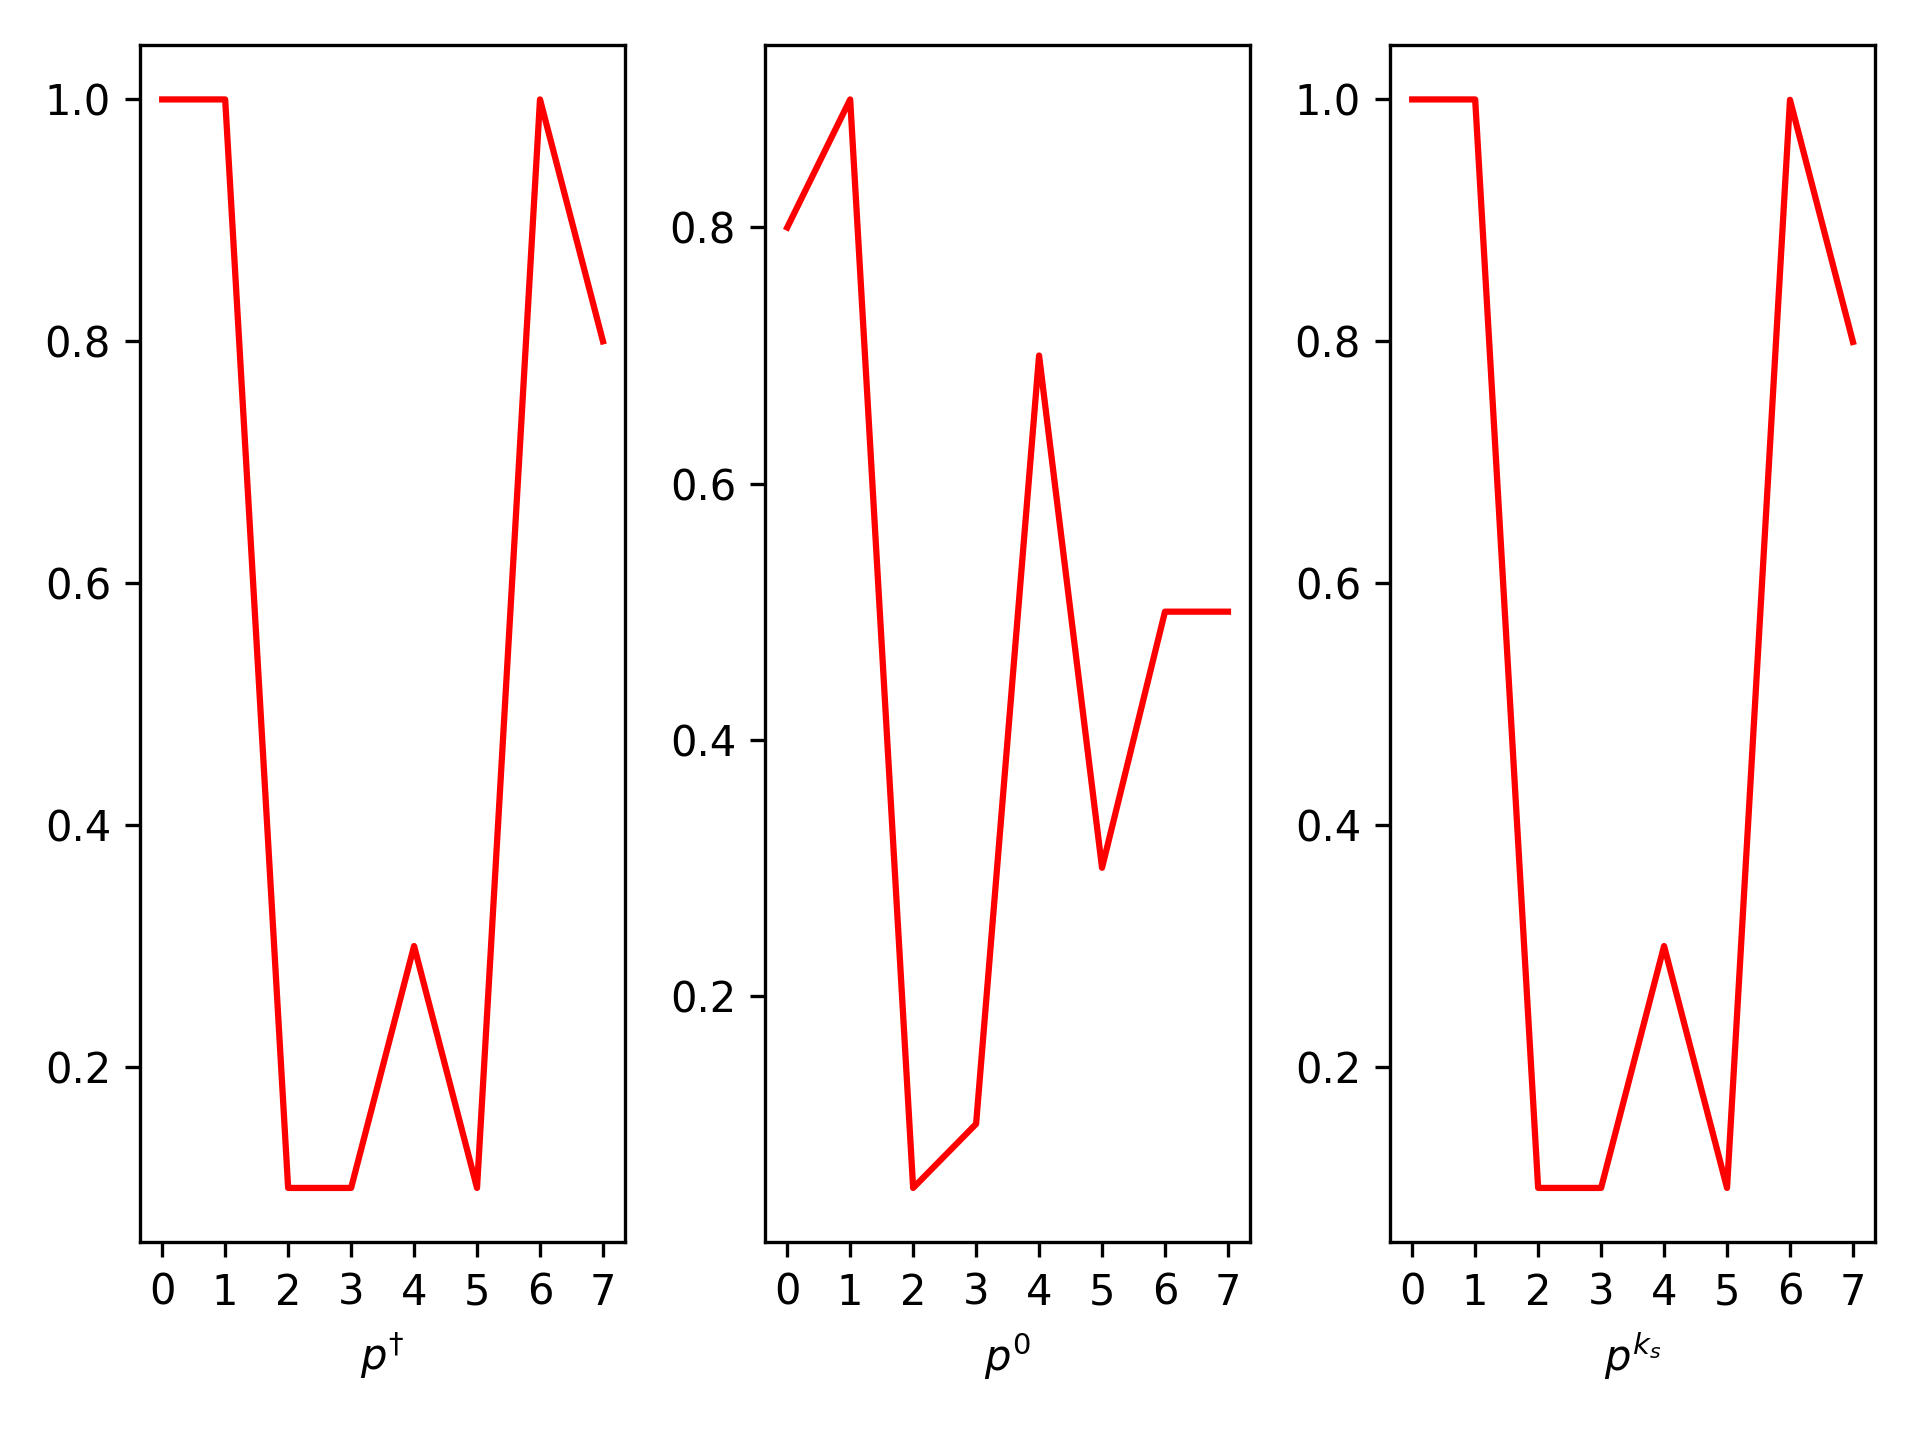
\includegraphics[width=0.8\textwidth]{./pics/gn_coeff.png}
    \caption{Coefficients, left truth, middle starting point, right
    iteration stop}
    \label{fig: gn_coeff}
\end{figure}
The below figure shows the standard loss used for the breaking criterion and
the residual loss
\begin{align}
    \log \left( \frac{\|\Psi(\vec{p}\;^{k+1}) -
    \Psi^{\dagger}\|}{\|\Psi(\vec{p}\;^{k}) - \Psi^{\dagger}\|} \right)
\end{align}
\begin{figure}[H]
    \centering
    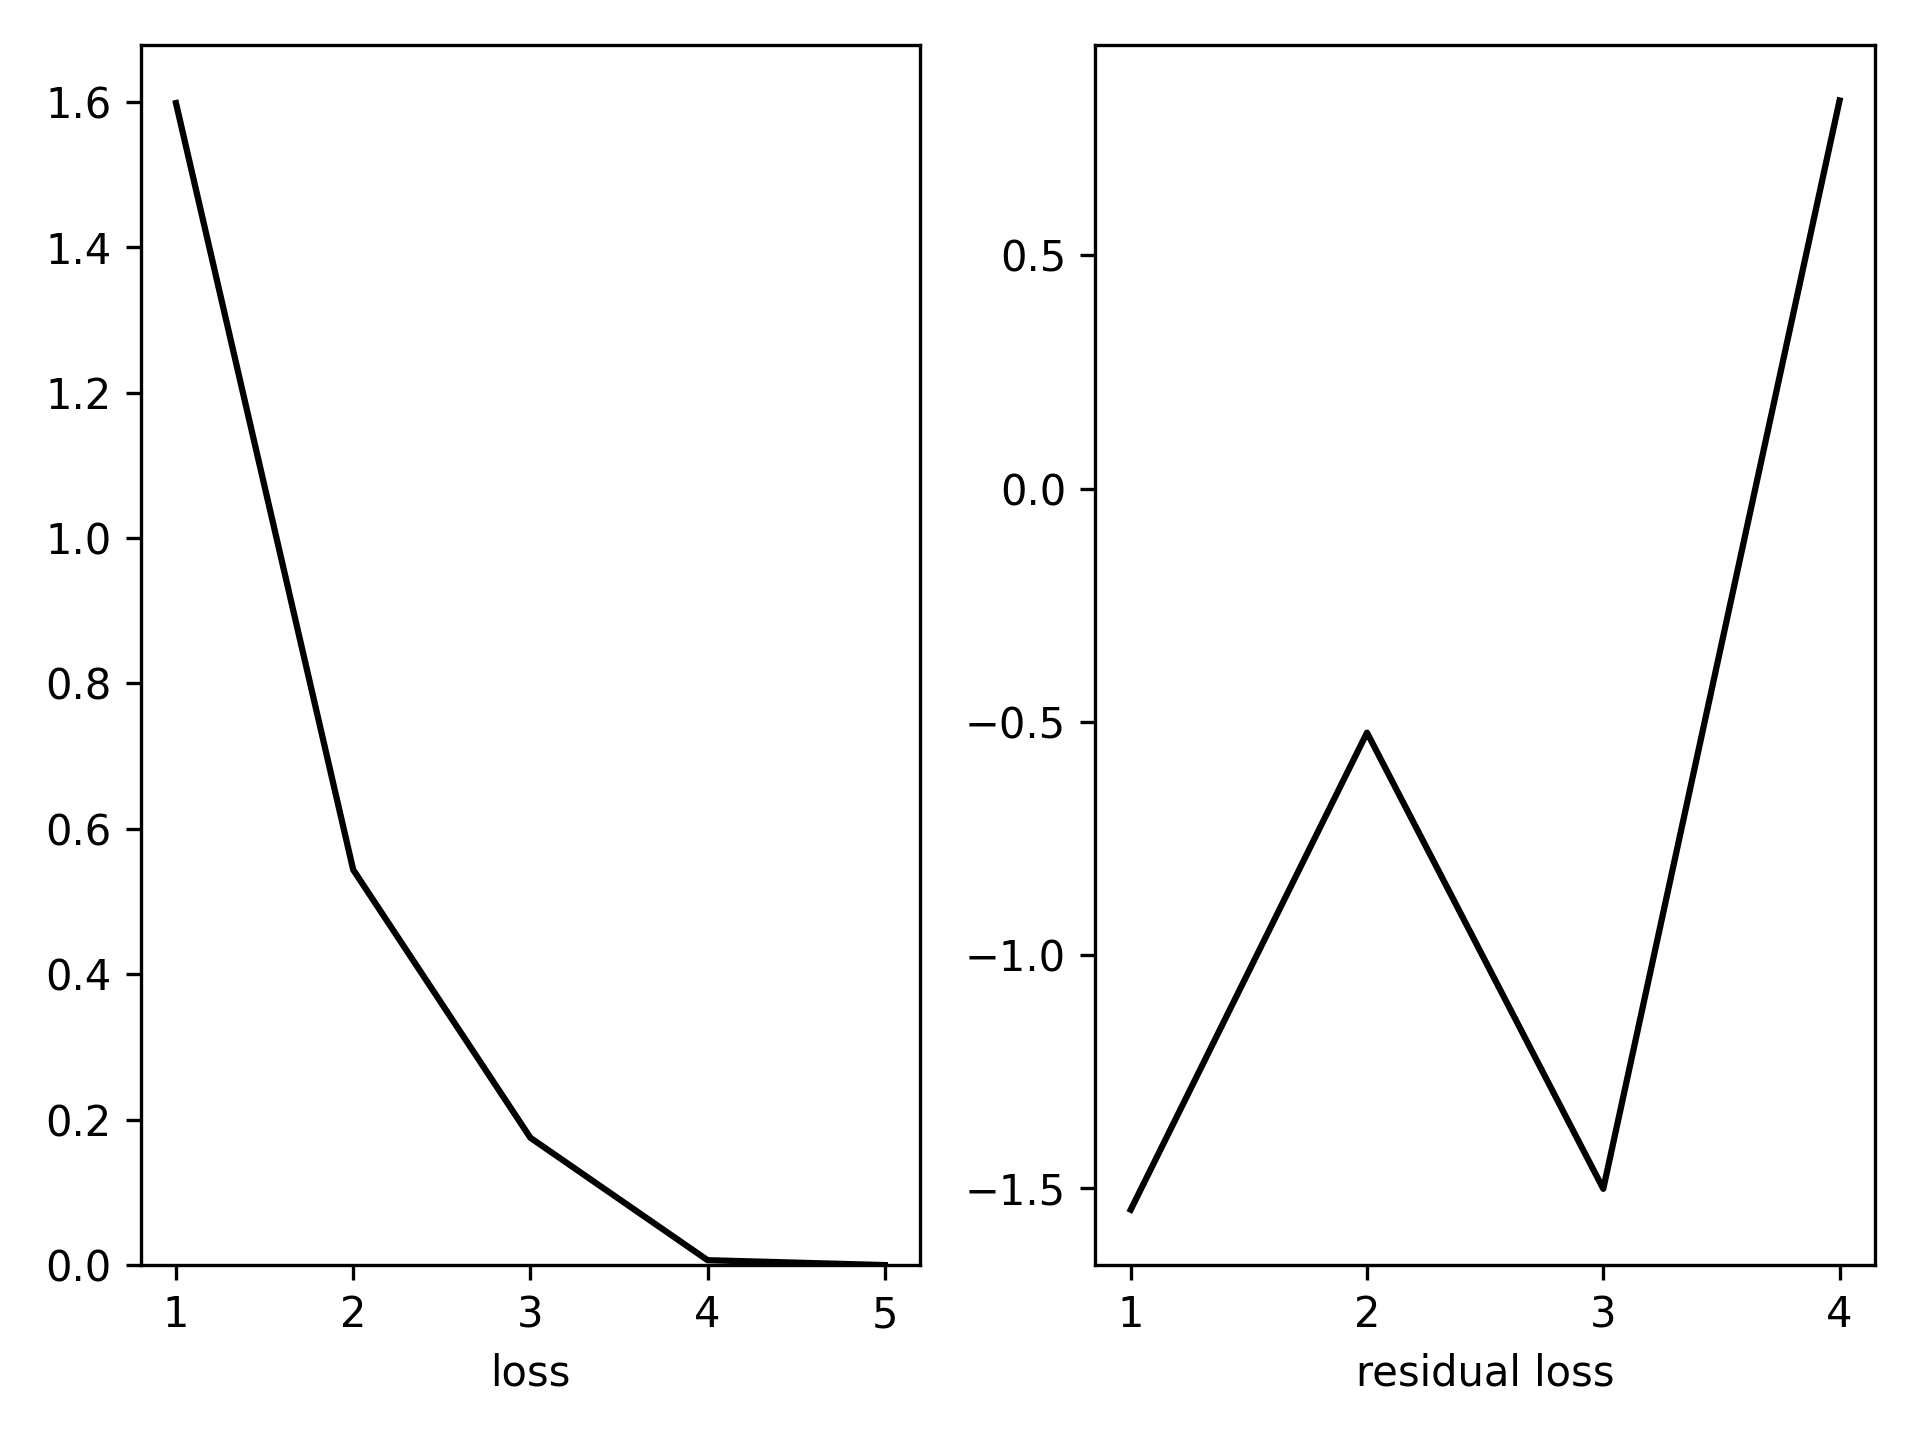
\includegraphics[width=0.8\textwidth]{./pics/gn_loss.png}
    \caption{Gauss-Newton loss, left standard norm loss, right residual loss}
    \label{fig: gn_loss}
\end{figure}


For comparison with the Gauss-Newton iteration, consider the Landweber iteration
\begin{align}
    \vec{p}\;^{k+1} = \vec{p}\;^{k} - \lambda \Psi'\left(\vec{p}\;^{k}  \right)^{\dagger}
    \left( \Psi(\vec{p}\;^{k}) - \Psi^{\dagger} \right) \qquad k \in
    \mathbb{N}_0.
\end{align}
Around $8000$ iteration are needed to reach the same accuracy that the
Gauss-Newton method reaches in $5$, with $\lambda = 0.02$ (e.g. $\lambda=0.2$
diverges).
\begin{figure}[H]
    \centering
    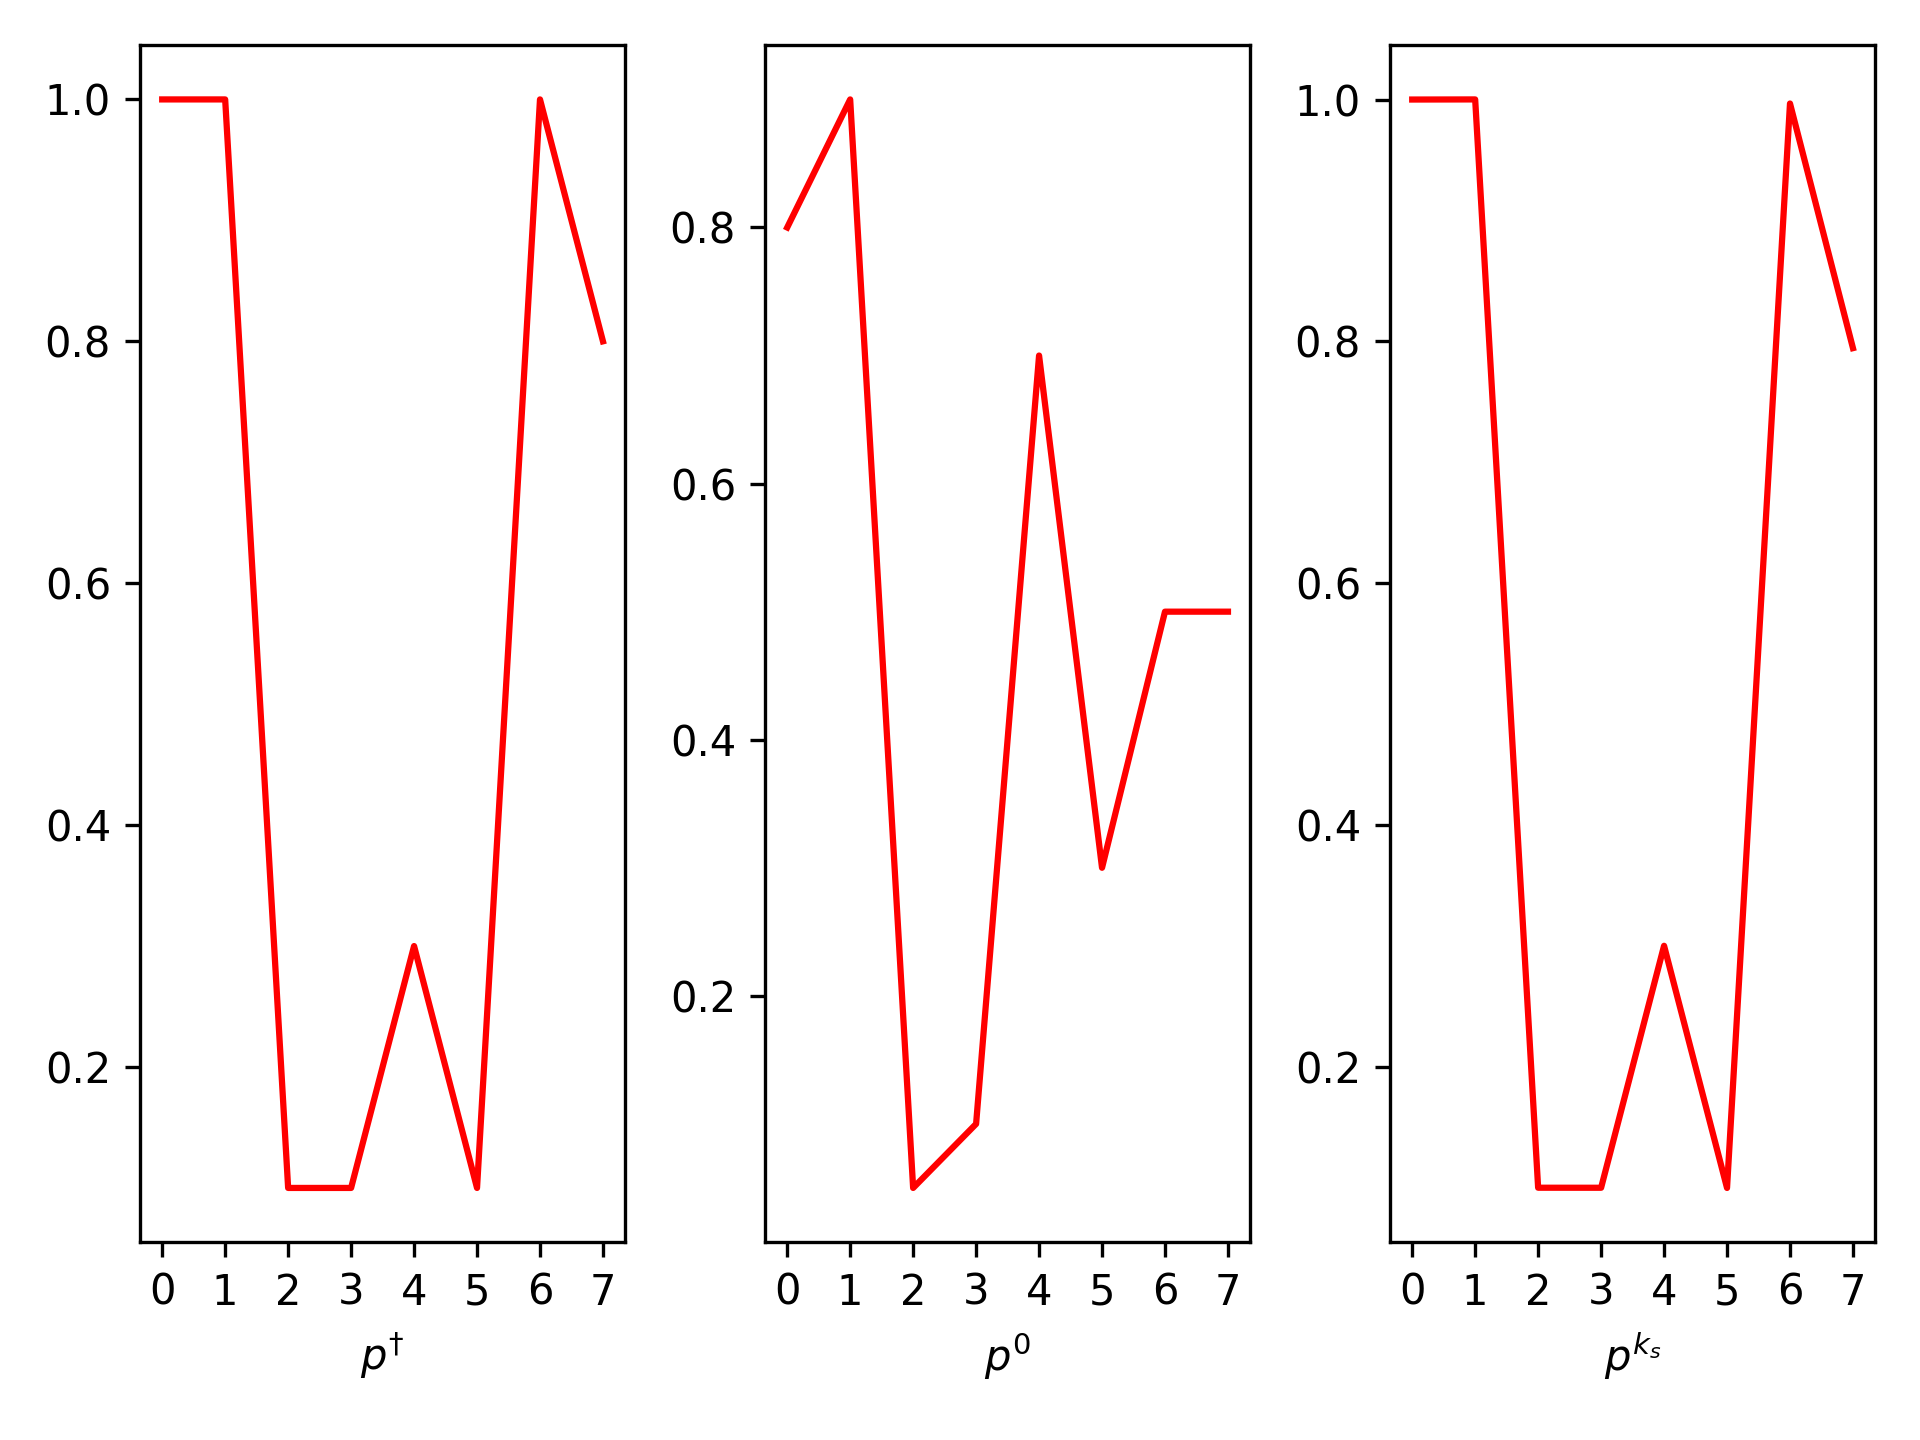
\includegraphics[width=0.8\textwidth]{./pics/lw_coeff.png}
    \caption{Coefficients, left truth, middle starting point, right
    iteration stop}
    \label{fig: lw_coeff}
\end{figure}
\begin{figure}[H]
    \centering
    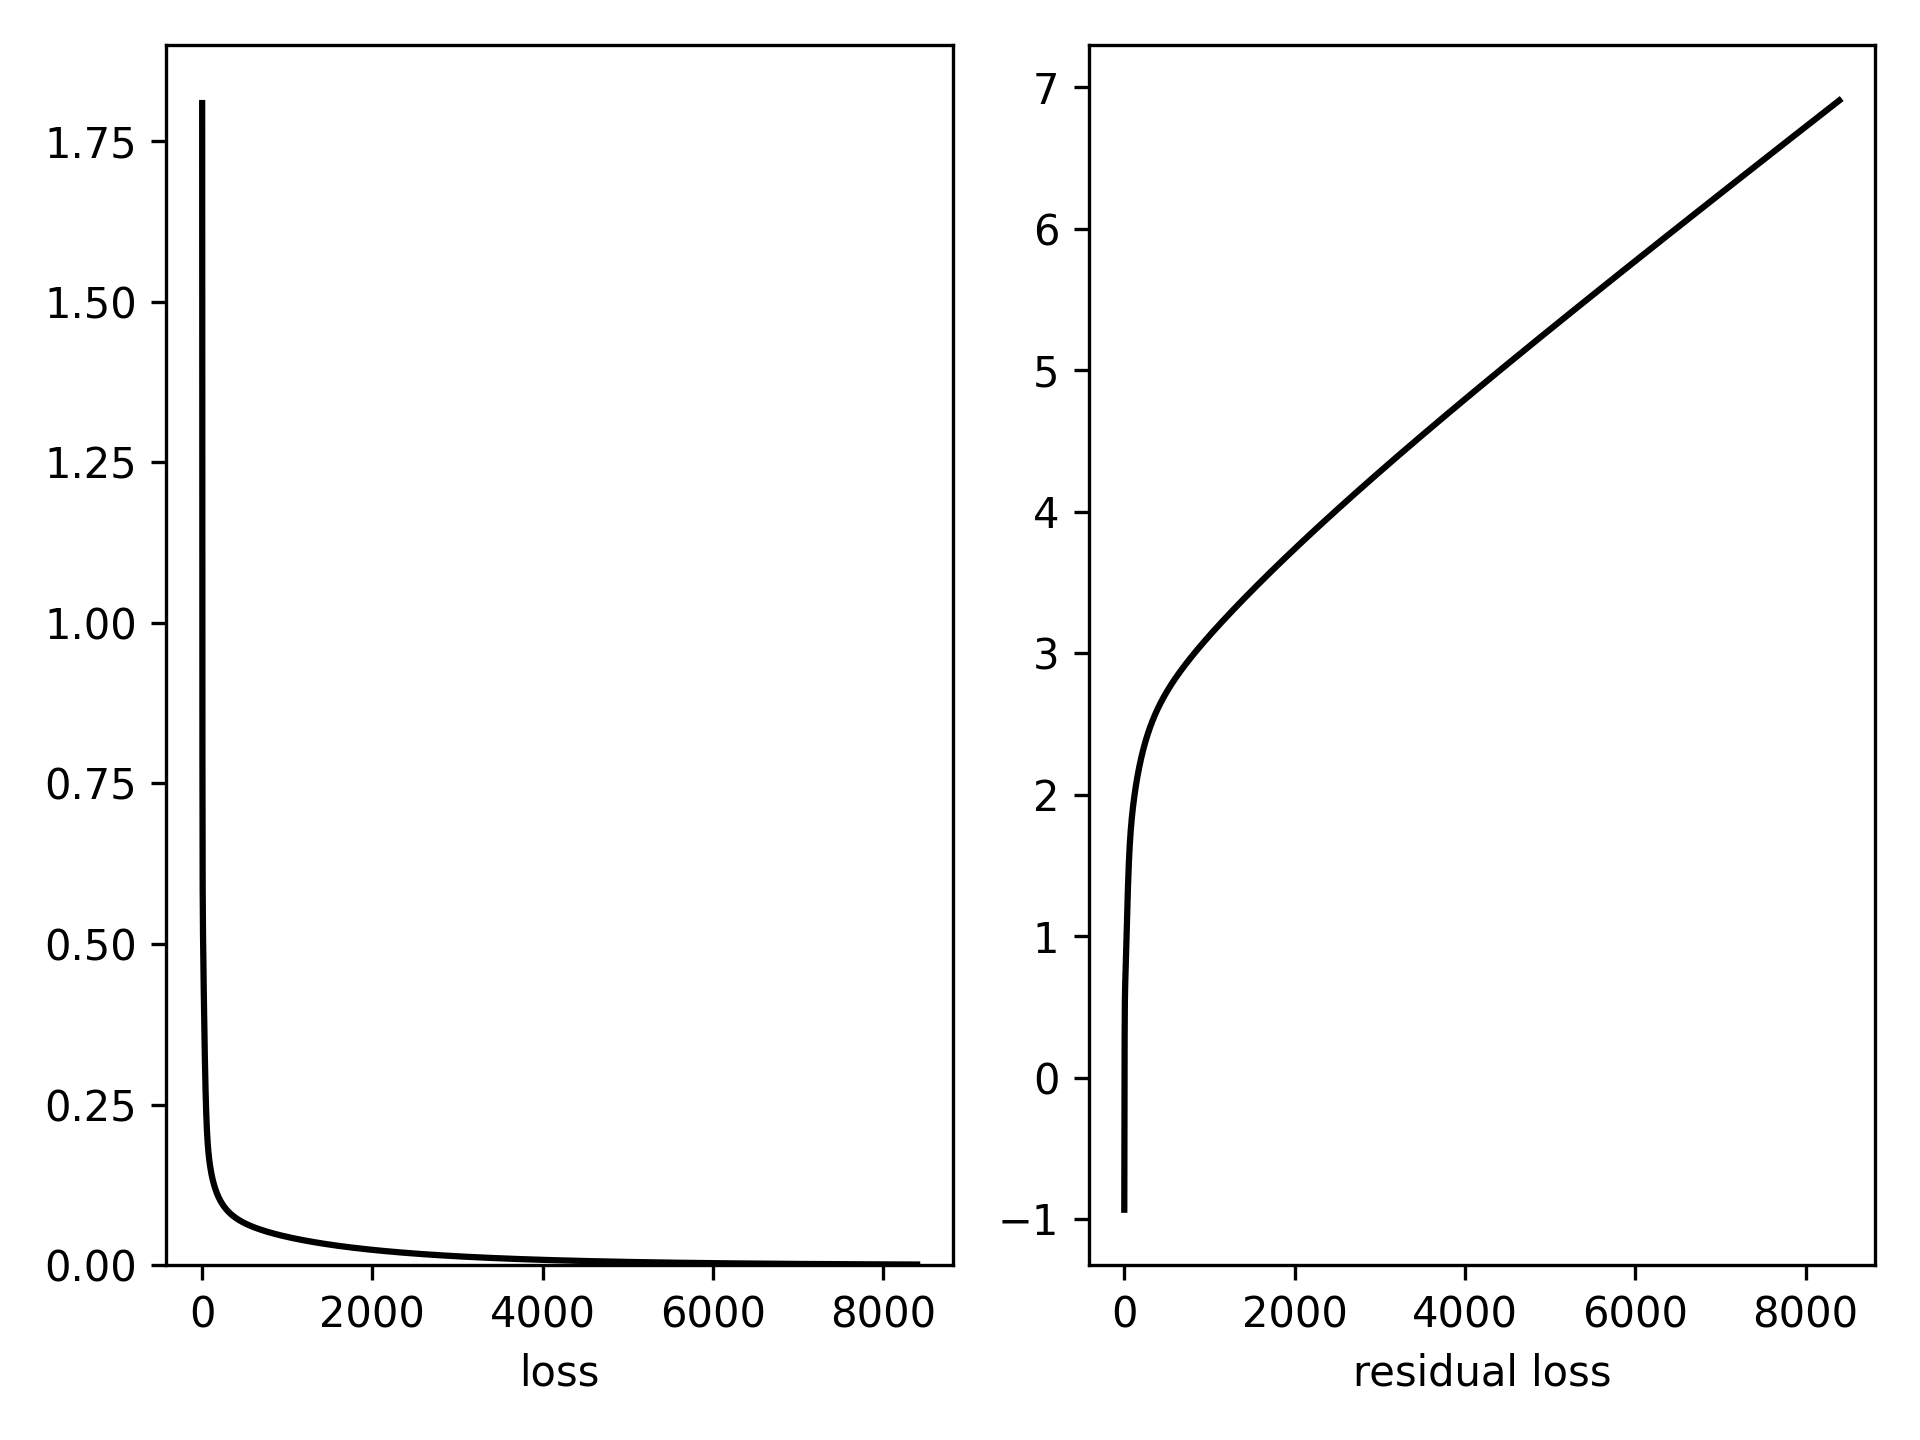
\includegraphics[width=0.8\textwidth]{./pics/lw_loss.png}
    \caption{Landweber loss, left standard norm loss, right residual loss}
    \label{fig: lw_loss}
\end{figure}

If the observed convergence rate of the Gauss-Newton can change completely if the
solution is not attainable. Then the conjecture is that the non-convergence
because of multiple solutions, which can be observed when not using enough
reconstruction data.
Also the implementation of the simplified Gauss-Newton requires inversion of
$F$ , which is not done in practice, this is not true for Landweber.
\subsection{Alternative to DNNs}
Instead of using Deep Neural Networks where it is unknown if
the immersion is invertible, another considerable option is to use
Quadratic neural network functions defined as follows
\begin{align}
    \Psi(\vec{x}) := \sum_{j=1}^{N} \alpha_j\sigma\left(\vec{x}^{T}A_j\vec{x}
        + \mathbf{w}_j^{T}\vec{x} + \theta_j \right),
\end{align}
with $\alpha_j, \theta_j \in \mathbb{R}, \mathbf{w}_j \in \mathbb{R}^{n}$
and $A_j \in \mathbb{R}^{n \times n}$. We can also constrain the class of
$A_j$ and $\mathbf{w}_j$ which leads us to circular networks, circular
affine, elliptic, parabolic...
\begin{theorem}
    Quadratic neural network functions satisfy the universal approximation
    property.
\end{theorem}
The immersion property of circular network functions
\begin{align}
    \Psi(\vec{x}) := \sum_{j=1}^{N} \alpha_j\sigma\left(r_j\vec{x}^{T}\vec{x}
        + \mathbf{w}_j^{T}\vec{x} + \theta_j \right),
\end{align}
and
\begin{align}
    \text{span}\{\partial_{p_i}\Psi(\vec{p})\;:\;i=1,\ldots,n_*\}, \qquad
    \text{has rank}(n_*).
\end{align}
For $\alpha_i \neq 0$, this in particular requires that the functions
\begin{align}
    \frac{\partial \Psi}{\partial r_s}  = \sigma\left( \rho \right)
    \vec{x}^{T}\vec{x}, \quad
    \frac{\partial \Psi}{\partial \alpha_s}  = \sigma\left( \rho \right)
    , \quad
    \frac{\partial \Psi}{\partial w_s^{t}}  = \sigma'\left( \rho \right)
    x_t,\quad
    \frac{\partial \Psi}{\partial \theta_s}  = \sigma'\left( \rho \right)
\end{align}
are \textbf{linearly independent}.
\newline

Results of these types of networks is that the Shepp-Logan can be represented
with \textbf{10 nodes} with elliptic neurons and \textbf{one layer}. Where as
for affine networks, both shallow and deep we need infinity neurons.

\appendix
\section{Proofs}
The following section is dedicated to fill the proofs to the theorems and
lemmas in the main text.
\begin{myproof}{Theorem \ref{thm: moore-penrose}}
    \label{proof: thm-moore-penrose}
    \begin{enumerate}
        \item To show that $\Psi'(\vec{p}\;)^{\dagger}$ is indeed the
            Moore-Penrose inverse we need to verify the four identities given
            in \ref{eq: moore-penrose}. Aligning the notation in the
            difinition of the Moore-Penrose inverse then
            \begin{align}
                &L = \Psi'(\vec{p}\;) : \vec{P}=\mathbb{R}^{n_*} \to
                \mathbf{X}, \\
                & B = \Psi'(\vec{p}\;)^{\dagger}: \mathbf{X} \to \vec{P}, \\
                &\mathcal{D}(B) = \mathcal{D}(\Psi'(\vec{p}\;)^{\dagger}) =
                \mathbf{X}, \\
                &P: \vec{P} \to \vec{P} \qquad \text{the zero operator},\\
                &Q = P_{\vec{p}}:\mathbf{X} \to \mathbf{X}_{\vec{p}}
                \qquad \text{the projection operator to }
                \mathbf{X}_{\vec{p}}.
            \end{align}
            For the third identity with $P = 0$, let $\vec{q} =
            (q_i)_{i=1}^{n_*} \in \vec{P}$ and we have
            \begin{align}
                \Psi'(\vec{p}\;)^{\dagger}\Psi'(\vec{p}\;)\vec{q} &=
                \Psi'(\vec{p}\;)^{-1}\left( \sum_{i=1}^{n_*} q_i
                \partial_{p_i} \Psi(\vec{p}\;) \right) \\
              &=\left(q_i  \right)_{i=1}^{n_*}  \\
              &= \vec{q}.
            \end{align}
            The fourth identity we use the fact that $(\partial_{p}
            \Psi(\vec{p}\;))_{i=1}^{n_*}$ is a basis, so for all $\mathbf{x}
            = (\mathbf{x_1}, \mathbf{x_2}) \in \mathbf{X}$ there exists an
            $x_i$, $i \in \{1,\ldots,n_*\}$ such that we can represent any
            $\mathbf{x}$ through
            \begin{align}
                \mathbf{x} = \sum_{i=1}^{n_*}
                x_i\partial_{p_i}\Psi(\vec{p}\;) + \mathbf{x_2},
            \end{align}
        with $\mathbf{x}_2 \in \mathbf{X}^{\perp}_{\vec{p}}$. Meaning that
        \begin{align}
            P_{\vec{p}}\;\mathbf{x} = \sum_{i=1}^{n_*} x_i\partial_{p_i}
            \Psi'(\vec{p}\;) \qquad \text{and},\\
            \Psi'(\vec{p}\;)^{\dagger}\mathbf{x} = (x_i)_{i=1}^{n_*}=\vec{x}.
        \end{align}
        Then the identity falls down to
        \begin{align}
            \Psi'(\vec{p}\;)\Psi'(\vec{p}\;)^{\dagger}\mathbf{x} =
            \Psi'(\vec{p}\;)\vec{x} = P_{\vec{p}}\;\vec{x}
        \end{align}
        For the second identity, use the results from the first and the
        fourth identity then fact that $\forall \mathbf{x} \in
        \mathbf{X}$:
        \begin{align}
            \Psi'(\vec{p}\;)^{\dagger}\Psi'(\vec{p}\;)
            \Psi'(\vec{p}\;)^{\dagger}\mathbf{x}
            &= \Psi'(\vec{p}\;)^{\dagger}
            \Psi'(\vec{p}\;)\vec{x} \\
            &= \vec{x}\\
            &= \Psi(\vec{p}\;)^{\dagger} \mathbf{x}.
        \end{align}
        For the first identity using the previous results $\forall \vec{q}
        \in \vec{P}$:
        \begin{align}
            \Psi'(\vec{p}\;)
            \Psi'(\vec{p}\;)^{\dagger}
            \Psi'(\vec{p}\;)
            &= \Psi'(\vec{p}\;) \vec{q}\\
            (&= L).
        \end{align}

        \item For the boundary constraint
    \end{enumerate}
\end{myproof}

\begin{myproof}{Lemma \ref{lem: moore-penrose}}
    \label{proof: lem-moore-penrose}
    \begin{enumerate}
        \item
            First of all by the chain rule it holds that
            \begin{align}
                N'(\vec{p}\;) = F\Psi'(\vec{p}\;) \qquad
                \forall \vec{p} \in \mathcal{D}(\Psi) = \mathcal{D}(N).
            \end{align}
            To prove the decomposition property of the Moore-Penrose
            inverse it is necessary to verify the equations
            \ref{eq: moore-penrose} defining it. With the notation
            \begin{align}
                &L:= N'(\vec{p}\;) = F\Psi'(\vec{p}\;): \vec{P} \to
                \mathbf{Y} \\
                &B:= \Psi'(\vec{p}\;)^{\dagger}F^{-1} : \mathcal{R}(F)
                \subseteq \mathbf{Y} \to \vec{P}.
            \end{align}
            Also note that by assumption $F$ has a dense range and consider
            $B$ on $\mathcal{R}(F) \dotplus
            \underbrace{\mathcal{R}(F)^{\perp}}_{=\{0\}}$. Thereby from for
            a fixed $\vec{p}$ the notation of \ref{eq: moore-penrose} is
            \begin{align}
                &\mathcal{D}(B) =
                \mathcal{D}(\Psi'(\vec{p}\;)^{\dagger}F^{-1}) =
                \mathcal{R}(F),\\
                &\mathcal{R}(L) = \big\{F\Psi'(\vec{p}\;)\vec{q}\;:\;\vec{q}
                \in \mathbb{R}^{n_*} \big\} = \mathcal{R}(FP_{\vec{p}}).
            \end{align}
            Note that $Q$ is an orthogonal projection onto
            $\overline{\mathcal{R}(L)}$, i.e.
            $\overline{\mathcal{R}(FP_{\vec{p}})}$, then for
            \begin{align}
                \mathbf{z} &= F\mathbf{x} \\
                    &= FP_{\vec{p}}\;
                    \mathbf{x} + F\left(I-P_{\vec{p}} \right) \mathbf{x}
            \end{align}
            we have that
            \begin{align}
                Q\mathbf{z} &= Q\left(FP_{\vec{p}}\;\mathbf{x}
                   + F(I-P_{\vec{p}})(\mathbf{x})\right) \\
                &= FP_{\vec{p}}\; \mathbf{x}.
            \end{align}
            Finally applying Lemma \ref{thm: moore-penrose} and the
            invertability of $F$ on the range of $F$ shows that
            \begin{align}
                LBL &= F\Psi'(\vec{p}\;)\Psi'(\vec{p}\;)^{\dagger}
                F^{-1}F\Psi'(\vec{p}\;) \\
                    &=
                    F\Psi'(\vec{p}\;)
                    \Psi'(\vec{p}\;)^{\dagger}\Psi'(\vec{p}\;) \nonumber\\
                    &= F \Psi'(\vec{p}\;) \nonumber \\
                    &= L \nonumber \\
                    \nonumber \\
                BLB &= \Psi'(\vec{p}\;)^{\dagger}F^{-1}F\Psi'(\vec{p}\;)
                \Psi'(\vec{p}\;)^{\dagger}F^{-1} \\
                    &=
                    \Psi'(\vec{p}\;)^{\dagger}
                    \Psi'(\vec{p}\;)\Psi'(\vec{p}\;)^{\dagger}F^{-1} \nonumber\\
                    &= \Psi'(\vec{p}\;)^{\dagger}F^{-1} \nonumber \\
                    &= B \nonumber \\
                    \nonumber \\
                BL &= \Psi'(\vec{p}\;)^{\dagger}F^{-1}F\Psi'(\vec{p}\;) \\
                   &= I - P \\
                   &= I \quad \text{on }  \mathbb{R}^{n_*}.
            \end{align}
            The fourth identity is proven by taking a $\mathbf{z} \in
            \mathcal{R}(F)$, so there exists a $\mathbf{x} \in \mathbf{X}$
            such that $F\mathbf{x} = \mathbf{z}$, then it follows
            \begin{align}
                LB\mathbf{z} &=
                F\Psi'(\vec{p}\;)\Psi'(\vec{p}\;)^{\dagger}
                F^{-1}\mathbf{z} \\
                 &= F\Psi'(\vec{p}\;)\Psi'(\vec{p}\;)^{\dagger}
                     \mathbf{x} \\
                &= FP_{\vec{p}}\mathbf{x} \\
                &= Q\mathbf{z}.
            \end{align}
        \item As for the generalized Newton-Mysovskii conditions, the
            operator $\Psi'(\vec{p})$ is locally bounded and locally
            Lipschitz continuous on $\mathcal{D}(\Psi)$, meaning that there are
            constants $C_L, C_l > 0$ such that $\forall \vec{p}, \vec{q} \in
            \mathcal{D}(\Psi)$ the following inequalities hold
            \begin{align}
                &\big\|\Psi'(\vec{p}\;) - \Psi'(\vec{q}\;)
                \big\|_{\vec{P}\to\mathbf{X}} \leq C_L \|\vec{p} - \vec{q} \|
                \\
                &\big\|\Psi'(\vec{p}) \big\|_{\vec{P} \to \mathbf{X}} \le
                C_l.
            \end{align}
            Thus
            \begin{align}
                &\Big\| N'(\vec{p}\;)^{\dagger}\left( N'(\vec{q} + s(\vec{p} -
                \vec{q}\;) - N'(\vec{q}\;)\right)
                (\vec{p} - \vec{q}) \Big\|_{\vec{P}} \\
                &= \Big\|
                \Psi'(\vec{p}\;)^{\dagger}F^{-1}\left( F\Psi'(\vec{q}\;
                + s\left( \vec{p} - \vec{q}\; \right)-F\Psi'(\vec{q}\;)
            \right)) \left(\vec{p} - \vec{q}  \right) \Big\|_{\vec{P}}
            \nonumber \\
                &= \Big\|
                \Psi'(\vec{p}\;)^{\dagger}\left(\Psi'(\vec{q}\;
                + s\left( \vec{p} - \vec{q}\; \right)-F\Psi'(\vec{q}\;)
            \right)) \left(\vec{p} - \vec{q}  \right) \Big\|_{\vec{P}}
            \nonumber\\
                &\leq C_lC_L s \|\vec{p} - \vec{q} \|^{2}_{\vec{P}},
                \nonumber
            \end{align}
        for all $\vec{p}, \vec{q} \in \mathcal{D}(\Psi) = \mathcal{D}(N)$.

    \end{enumerate}

\end{myproof}

\begin{myproof}{Theorem \ref{thm: gauss-newton-convergence}}
    \label{proof: thm-gauss-newton-convergence}
    The distance to the solution and the first iterate is $\rho =
    \|\vec{p}\;^{\dagger} - \vec{p}\;^{0}\|$. Also $\mathcal{D}(\Psi) =
    \mathcal{D}(N)$ since $F$ is defined all over $\mathcal{X}$. First of all
    we have to prove that all iterates lie in the closed ball, i.e.
    $\vec{p}\;^{k} \in \overline{\mathcal{B}(\vec{p}\;^{\dagger}; \rho)}$.,
    this is done by induction. The case $k=0$ is fulfilled by the existence assumption.
    For $\vec{p}\;^{k}$ use the equations \ref{eq: moore-penrose}
    \begin{align}
        &N'(\vec{p}\;^{k})N'(\vec{p}\;^{k})^{\dagger}N'(\vec{p}\;^{k})
        \left(\vec{p}\;^{k+1} - \vec{p}\;^{\dagger}  \right)\\
        &= N'(\vec{p}\;^{k})(\vec{p}\;^{k+1} - \vec{p}\;^{k}).
    \end{align}
    Then the definition of the Gauss-Newton method
    \ref{eq: gauss-newton-iteration} implies
    \begin{align}
        &N'(\vec{p}\;^{k})(\vec{p}\;^{k+1}-\vec{p}\;^{\dagger}) =\\
        &=N'(\vec{p}\;^{k})N'(\vec{p}\;^{k})^{\dagger}\left(
        N(\vec{p}\;^{\dagger})-N(\vec{p}\;^{k})
        - N'(\vec{p}\;^{k})(\vec{p}\;^{\dagger} - \vec{p}\;^{k})\right) .
    \end{align}
    Now using the third identity in \ref{eq: moore-penrose}, by the assumption
    of this theorem $P = 0$ and using the second identity in
    \ref{eq: moore-penrose} with the fact that $F$ is injective, it follows
    that
    \begin{align}
        \vec{p}\;^{k+1} - \vec{p}\;^{\dagger}
        &=
        N'(\vec{p}\;^{k})^{\dagger}N'(\vec{p}\;^{k})(\vec{p}\;^{k+1} -
        \vec{p}^{\dagger}) \\
        &=
        N'(\vec{p}\;^{k})^{\dagger}\left(N(\vec{p}\;^{\dagger})-N(\vec{p}\;^{k})
        - N'(\vec{p}\;^{k})(\vec{p}\;^{\dagger} - \vec{p}\;^{k}) \right) \\
        &= \Psi'(\vec{p}\;^{k})^{\dagger}\left(\Psi(\vec{p}\;^{\dagger}-
        \Psi(\vec{p}\;^{k}) -
    \Psi'(\vec{p}\;^{k})(\vec{p}\;^{\dagger}-\vec{p}\;^{k}) \right).
    \end{align}
    Finally the Newton-Mysovskii conditions give use
    \begin{align}
        \|\vec{p}\;^{k+1} - \vec{p}\;^{\dagger}\|
        &\le \frac{C_lC_L}{2}
        \|\vec{p}\;^{k} - \vec{p}\;^{\dagger}\|^{2}_{\vec{P}} \\
        &\le \frac{C_lC_L\rho}{2}
        \|\vec{p}\;^{k}-\vec{p}\;^{\dagger}\|_{\vec{P}} \\
        &< \|\vec{p}\;^{k} - \vec{p}\;^{\dagger}\|_{\vec{P}},
    \end{align}
    meaning that $\vec{p}\;^{k+1} \in \mathcal{B}(\vec{p}\;^{\dagger};
    \rho)$, thereby the Gauss-Newton method is well defined. Also
    \begin{align}
        \|\vec{p}\;^{k+1} - \vec{p}\;^{\dagger}\|
        &\leq \left( \frac{C_lC_L\rho}{2}  \right)^{k+1}
        \|\vec{p}\;^{0} - \vec{p}\;^{\dagger}\| \\
        &\le \left( \frac{C_lC_L\rho}{2}  \right)^{k+1} \rho,
    \end{align}
    where $\frac{C_lC_L\rho}{2} < 1$, meaning that the Gauss-Newton method
    converges to $0$ as $k\to \infty$, quadratically. \qed
\end{myproof}

\begin{myproof}{Lemma \ref{lemma: immersion}}
    \label{proof: lem-immersion}
    \begin{itemize}
        \item Because of the differentiability assumptions of $\sigma$, for
    all fixed $\vec{p}$, we have that $D\Psi[\vec{p}\;] \in
    L^{2}\left([0,1]^{n}\right)$. So the Conjecture \ref{conj: main} directly
    implies that $\mathcal{R}(D\Psi[\vec{p}\;])$ is a linear subspace of
    $\mathbf{X}$ of dimension $n_*$.
\item Note that the operator $D^{2}\Psi[\vec{p}\;]: \mathbb{R}^{n_*} \to
    L^{2}([0, 1]^{n})$ is continuous (assuming that the activation function
    $\sigma$ is twice differentiable. Considering a nonempty neighborhood
    $\mathcal{U}$ of $\vec{p}$ with a compact closure, the continuity of
    $D^{2}\Psi$ w.r.t $\vec{p}$ gives that $D\Psi$ is
    Fr\'echet-differentiable with Lipschitz-continuous derivative on
    $\mathcal{U}$. Meaning there exist constants $C_l, C_L > 0$ such that
    for all $\vec{q}, \vec{p} \in \mathcal{D}(\Psi)$ it holds that
        \begin{align}
            &\big\|\Psi'(\vec{p}\;) - \Psi'(\vec{q}\;)
            \big\|_{\vec{P}\to\mathbf{X}} \leq C_L \|\vec{p} - \vec{q} \|
            \\
            &\big\|\Psi'(\vec{p}) \big\|_{\vec{P} \to \mathbf{X}} \le
            C_l.
        \end{align}
        \qed
    \end{itemize}

\end{myproof}





\nocite{kaltenbacher2008}
\nocite{frischauf2022universal}
\printbibliography

\end{document}
